\chapter{Risultati}
Si riportano di seguito i principali risultati ottenuti in merito alle performance dell'algoritmo. 


\section{Hardware di riferimento}
L'algoritmo è stato eseguito su una macchina con le seguenti caratteristiche:

\begin{tabular}{>{\hspace{1em}}l l}
Sistema operativo & Ubuntu 20.04\\
Kernel & 5.15.0-52-generic\\
Processore & Intel Core i7-9750H @4.10GHz\\         
Ram & 16GB @2666MHz CL19\\
Python & 3.10\\
\end{tabular}

\section{Sudoku}

\subsection{Casi di test}
È stato usato come esempio di riferimento il problema della risoluzione di un sudoku per mostrare il variare delle prestazioni al variare delle righe della matrice A (N nei grafici): a parità di dimensione del sudoku infatti, il numero di colonne della matrice è uguale indipendentemente dalla percentuale di riempimento dello stesso. In questo caso specifico il sudoku scelto è di dimensione 9x9, che dà origine ad una matrice A con 384 colonne e in cui ciascuna riga ha esattamente 4 elementi pari a 1 e tutti gli altri a 0. Sono stati testati entrambi gli algoritmi, base e plus, con una percentuale di riempimento dal $80\%$ al $70\%$ con uno step del $2\%$, facendo la media su 5 run per ogni iterazione in modo da ridurre al minimo gli errori dovuti al possibile utilizzo della cpu di altre applicazioni in background. Queste percentuali sono state scelte perché si sono rivelate un buon compromesso tra la significatività del risultato temporale e la fattibilità dell'esecuzione, in quanto sopra $80\%$ i tempi risultano troppo brevi mentre sotto il $70\%$ troppo lunghi.

\subsection{Ottimizzazione specifica per il sudoku}
Come esposto nella sezione 2, è stata introdotta un'ottimizzazione specifica per il problema del sudoku che riduce le righe della matrice A. Nella figura \ref{row:opt} viene mostrata la riduzione avvenuta rispetto alle righe originali, da cui si evince una correlazione lineare tra le due. Questo è confermato anche dalla figura \ref{rate:row}, che mostra il numero di righe già ottimizzate rispetto al rateo del sudoku. Quest'ultima ci permette anche di valutare i tempi e i nodi visitati interscambiabilmente rispetto al numero di righe di A o rispetto al rateo del sudoku.

\begin{figure}[h!]
\centering
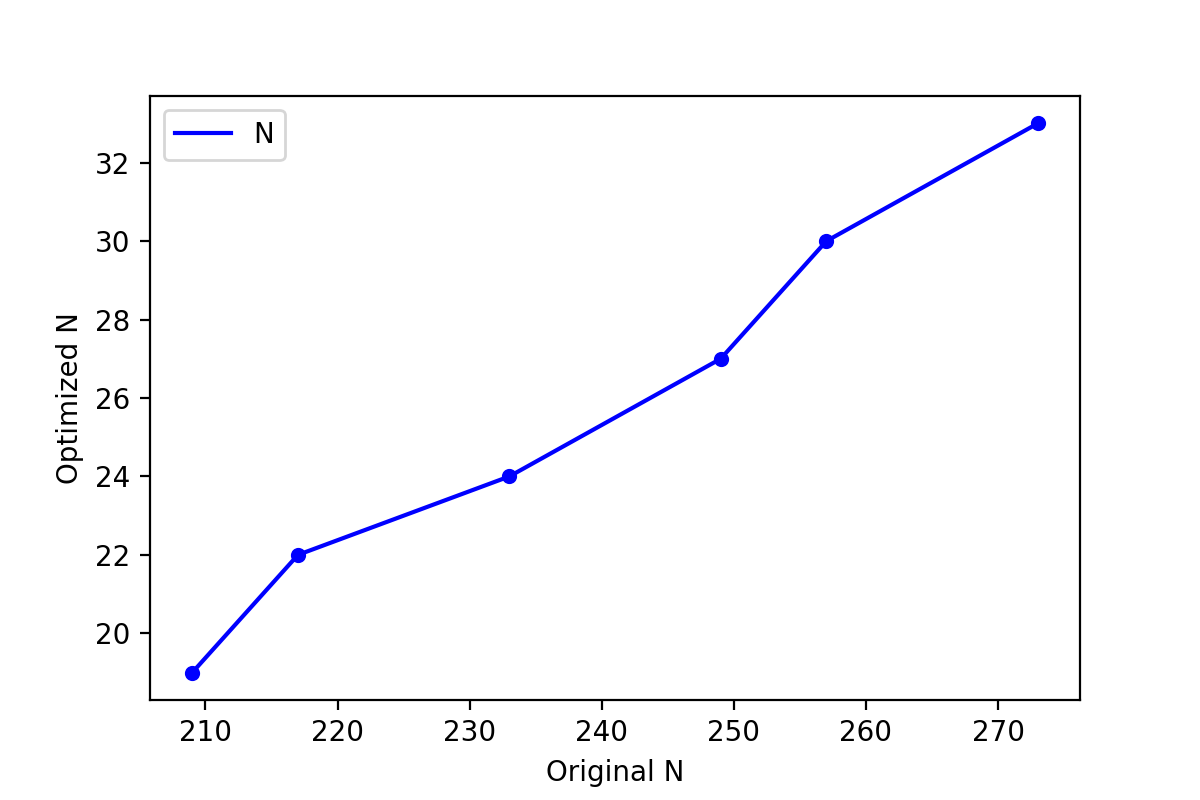
\includegraphics[width=0.8\linewidth]{figures/sudoku/s3_opt_row.png}
\caption{Riduzione delle righe della matrice A}\label{row:opt}
\end{figure}

\begin{figure}[h!]
\centering
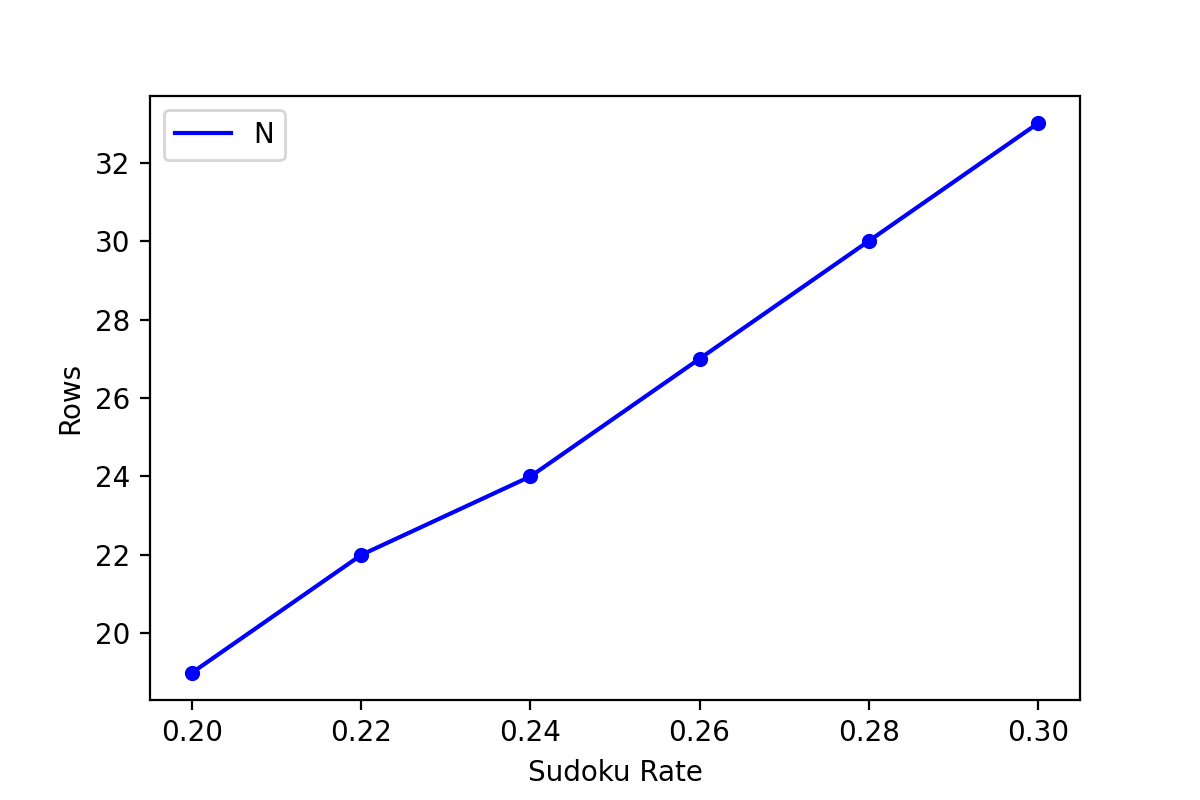
\includegraphics[width=0.8\linewidth]{figures/sudoku/s3_rate_row.png}
\caption{Rateo di riempimento del sudoku rispetto alle righe della matrice A}\label{rate:row}
\end{figure}

\subsection{Tempo di esecuzione}
Nella figura \ref{n:time} viene mostrata la performance temporale dell'algoritmo al variare delle righe della matrice A. Da questa si evince la crescita polinomiale del tempo di esecuzione. Si nota anche un grosso vantaggio della versione plus dell'algoritmo che aumenta all'aumentare di N.



\begin{figure}[h!]
\centering
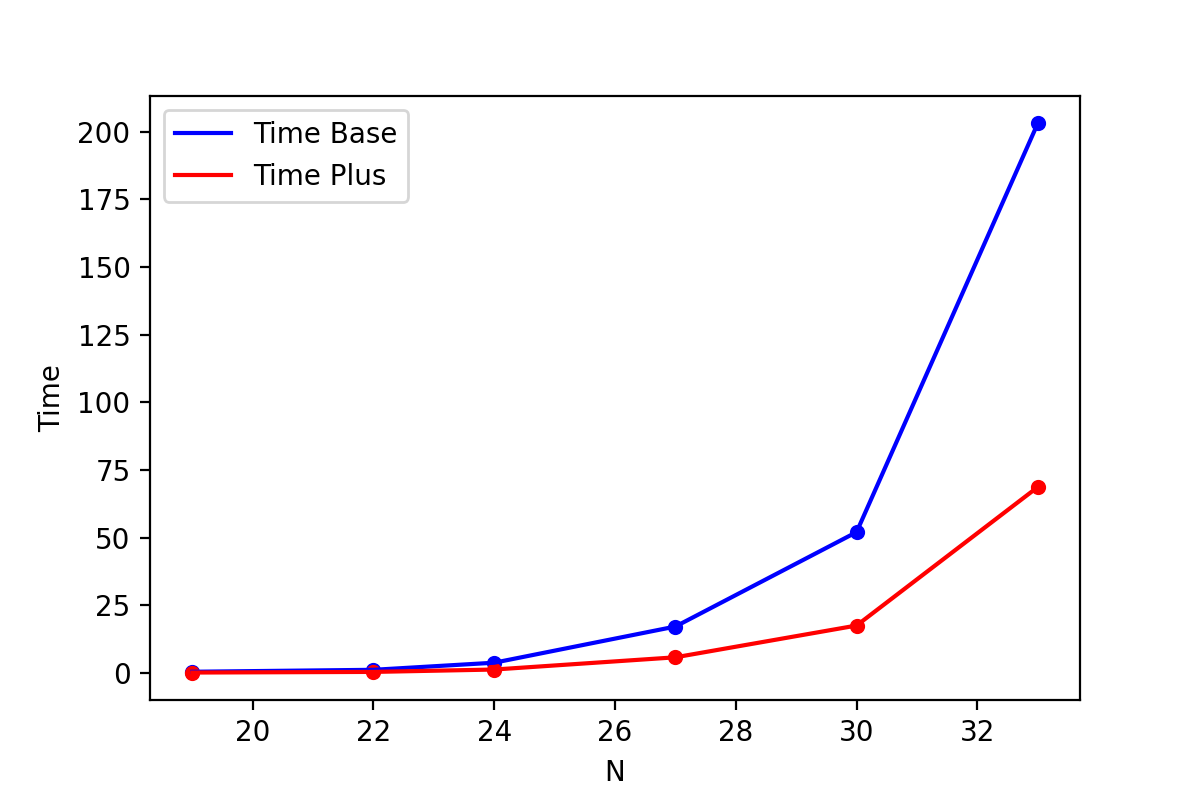
\includegraphics[width=0.8\linewidth]{figures/sudoku/s3_N_time.png}
\caption{Tempo al variare delle righe della matrice A}
\label{n:time}
\end{figure}

\subsection{Nodi visitati}
Nella figura \ref{row:nodes} viene mostrato il rapporto tra nodi totali dell'albero del problema confrontati con i nodi effettivamente visitati dall'algoritmo, rispetto all'aumentare di N. Essendo enormemente maggiori i primi, nella figura \ref{row:visited} vengono mostrati solamente i nodi visitati in modo da riuscire a coglierne l'andamento.


\begin{figure}[h!]
\centering
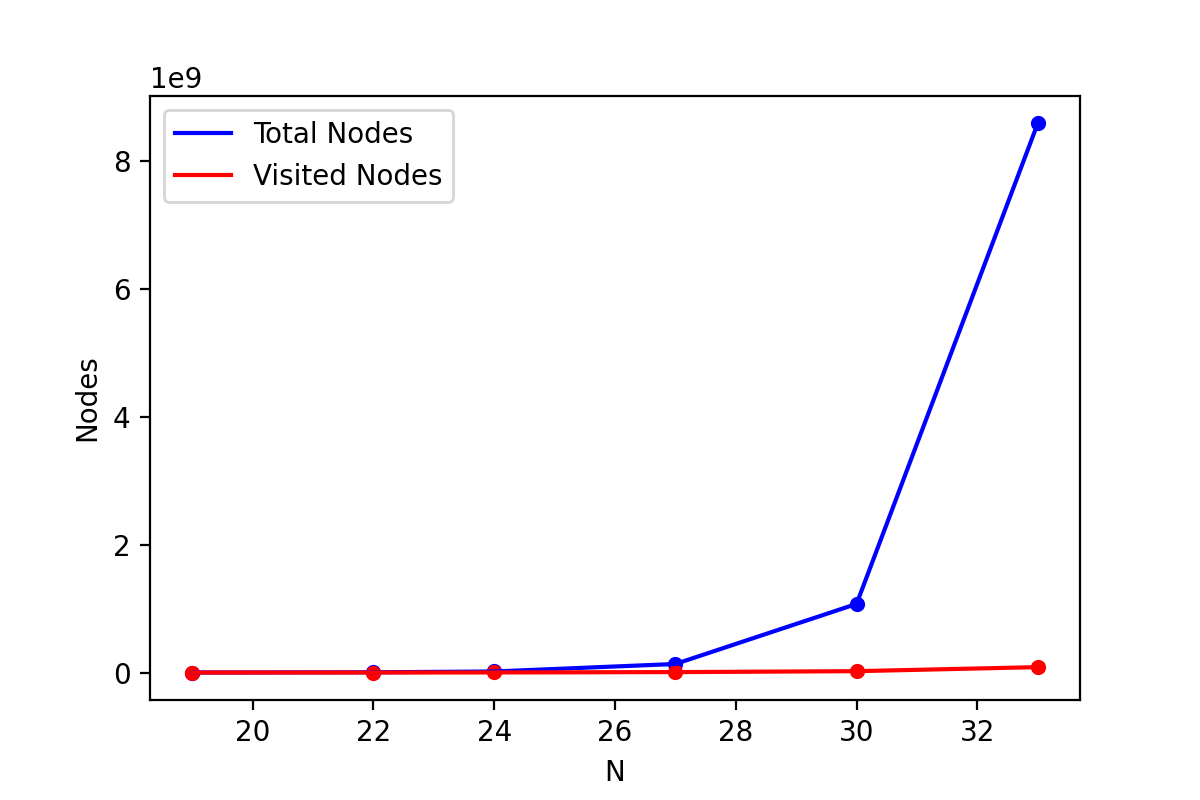
\includegraphics[width=0.8\linewidth]{figures/sudoku/s3_row_nodes.png}
\caption{Nodi totali e visitati al variare delle righe della matrice A}
\label{row:nodes}
\end{figure}


\begin{figure}[h!]
\centering
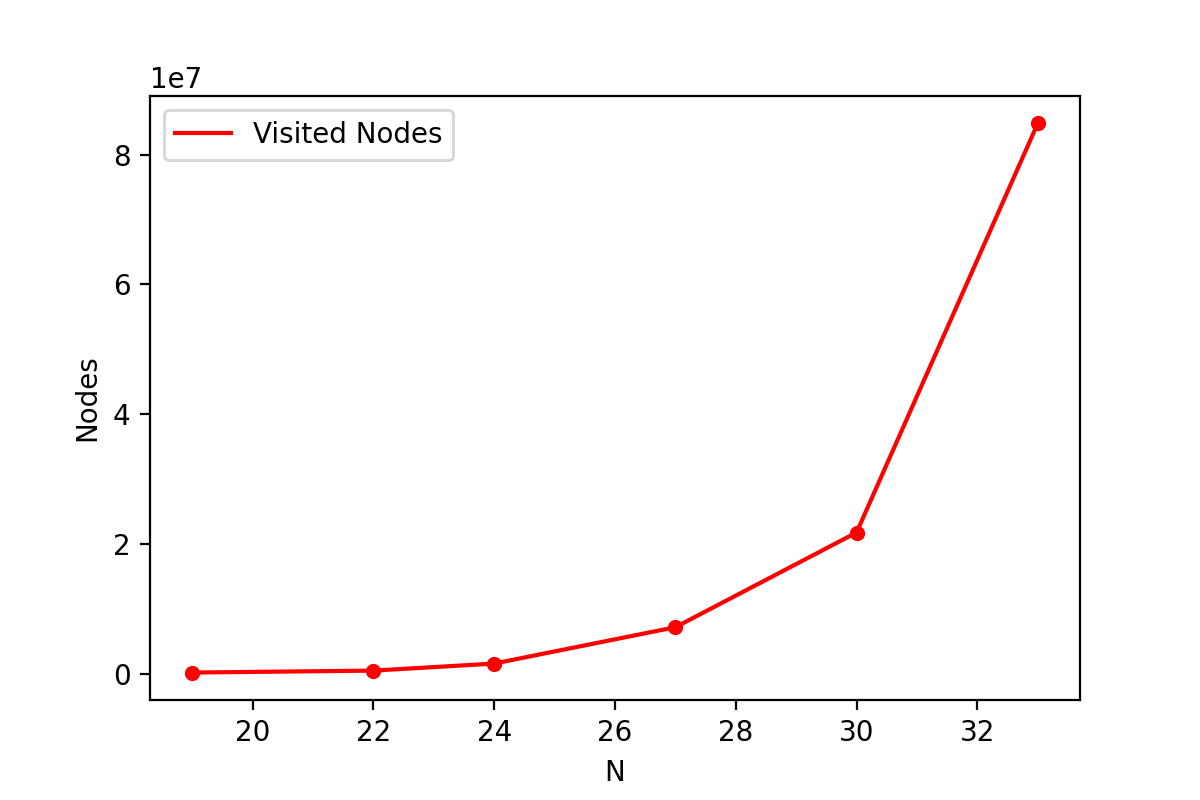
\includegraphics[width=0.8\linewidth]{figures/sudoku/s3_row_visited.png}
\caption{Nodi visitati al variare delle righe della matrice A}
\label{row:visited}
\end{figure}

\newpage{}

\subsection{Occupazione di memoria}
Nella figura \ref{row:mem} viene mostrata l'occupazione spaziale dell'algoritmo al variare della dimensione del problema in righe della matrice A, registrata profilando l'occupazione di memoria delle due funzioni che implementano lo stesso.

\begin{figure}[h!]
\centering
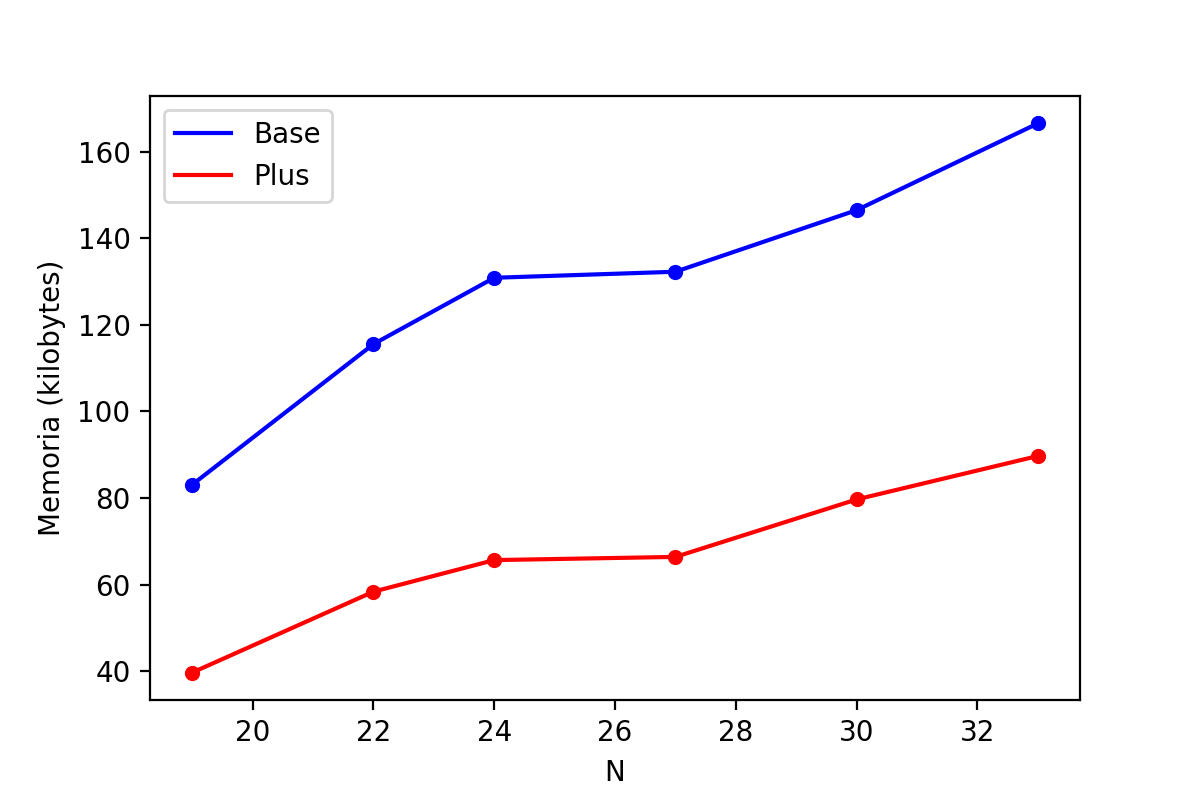
\includegraphics[width=0.8\linewidth]{figures/sudoku/s3_n_mem.png}
\caption{Occupazione spaziale dell'algoritmo al variare delle righe di A}
\label{row:mem}
\end{figure}


\newpage
\section{Random}

\subsection{Casi di test}
Siccome i casi di test creati per la risoluzione del sudoku mostrano l'andamento delle performance dell'algoritmo solo al variare delle righe, per completezza è stato testato l'algoritmo anche con matrici A create randomicamente in modo da mostrare la differenza di performance al variare delle colonne a parità di righe. Sono stati create 6 matrici A con 40 righe e colonne da 15 a 25 ed ognuna di esse è stata testata su 5 run facendo la media dei risultati. Come per il sudoku, la dimensione delle matrici è stata scelta dopo alcune prove empiriche come compromesso tra significatività dei risultati e fattibilità della computazione. È stata inoltre aggiunta una condizione opzionale che permette di assicurare sempre la presenza di almeno una soluzione nella matrice random creata, oltre a ciò non è stata eseguita alcuna ottimizzazione sull'input. Nella figura \ref{m:cov} viene mostrato il numero di soluzioni che diminuisce al crescere delle dimensioni del problema.

\begin{figure}[h!]
\centering
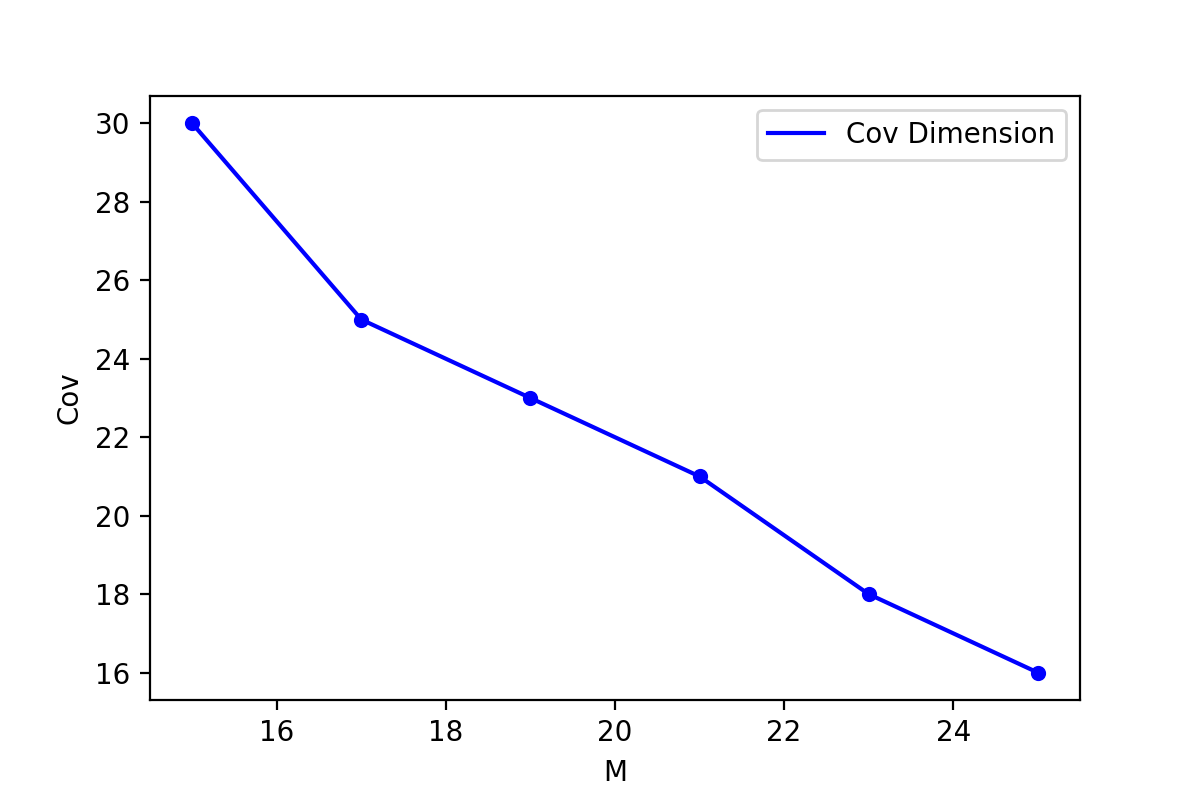
\includegraphics[width=0.9\linewidth]{figures/random/r_col_cov.png}
\caption{Numero di soluzioni al variare delle colonne della matrice A}
\label{m:cov}
\end{figure}


\subsection{Tempi di esecuzione}
Nella figura \ref{m:time} viene mostrata la performance temporale dell'algoritmo al variare delle colonne della matrice A. Da questa si evince la crescita polinomiale del tempo di esecuzione, come nel caso del sudoku. In questo caso la differenza di prestazioni tra le due vesioni dell'algoritmo è ridotta rispetto al sudoku ma si alza nel caso della versione che utilizza una stringa binaria per rappresentare la matrice.

\begin{figure}[h!]
\centering
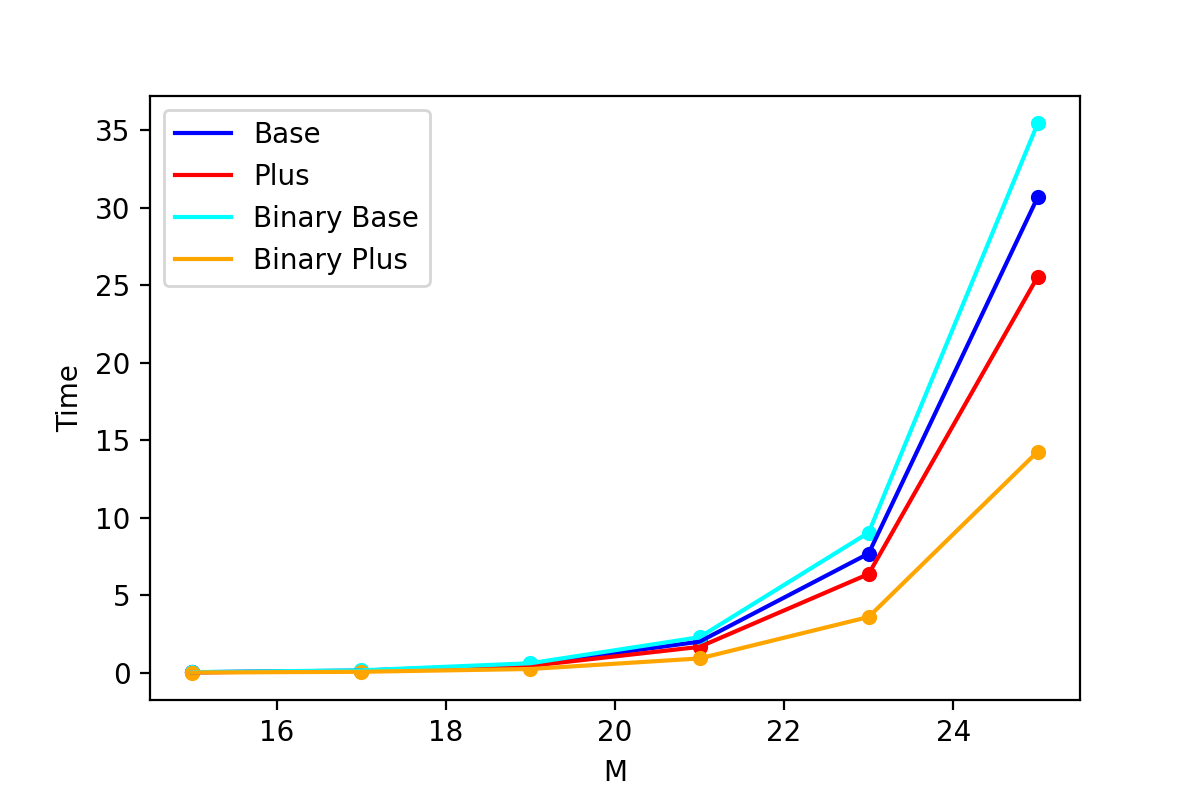
\includegraphics[width=0.8\linewidth]{figures/random/binary_time.png}
\caption{Tempo al variare delle colonne della matrice A}
\label{m:time}
\end{figure}

\newpage
\subsection{Nodi visitati}
Nella figura \ref{m:nodes} vengono mostrati i nodi dell'albero del problema visitati dall'algoritmo.

\begin{figure}[h!]
\centering
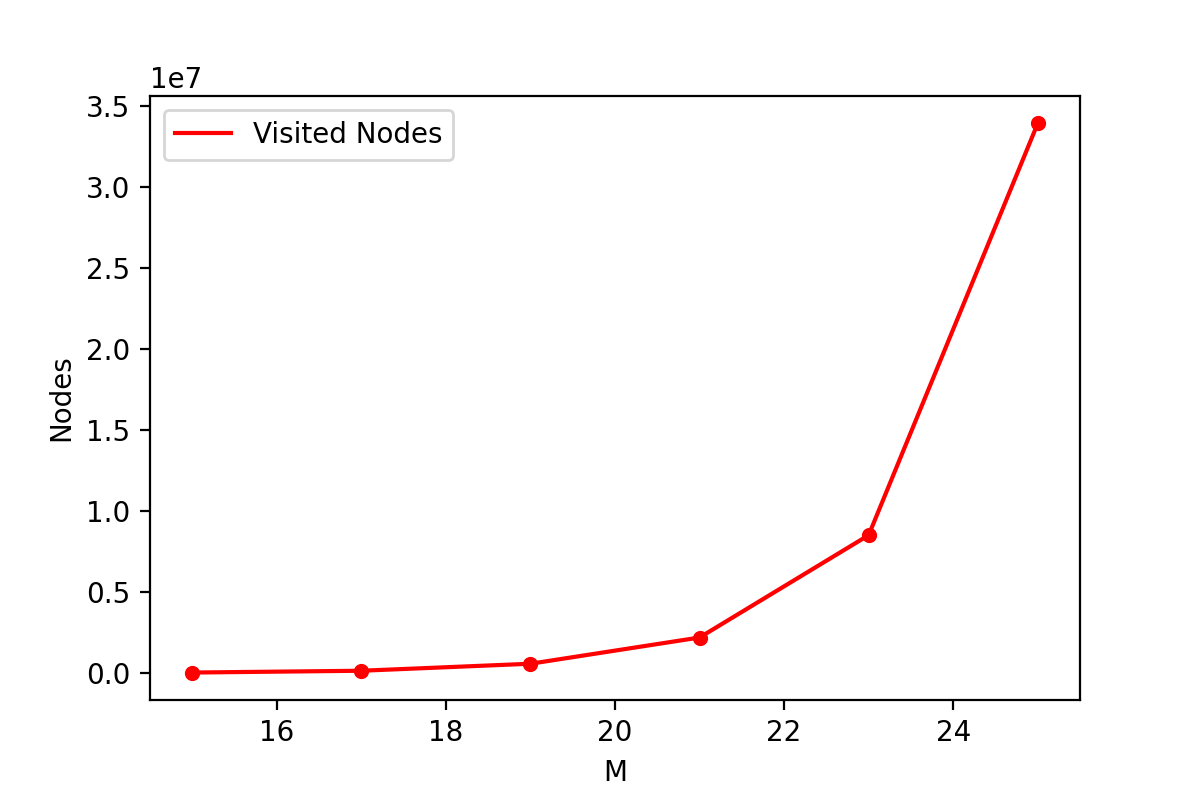
\includegraphics[width=0.8\linewidth]{figures/random/r_col_nodes.png}
\caption{Nodi visitati al variare delle colonne della matrice A}
\label{m:nodes}
\end{figure}

\newpage

\subsection{Occupazione di memoria}
Nella figura \ref{row:mem:r} viene mostrata l'occupazione spaziale dell'algoritmo al variare della dimensione del problema in colonne della matrice A, registrata profilando l'occupazione di memoria delle due funzioni che implementano lo stesso.

\begin{figure}[h!]
\centering
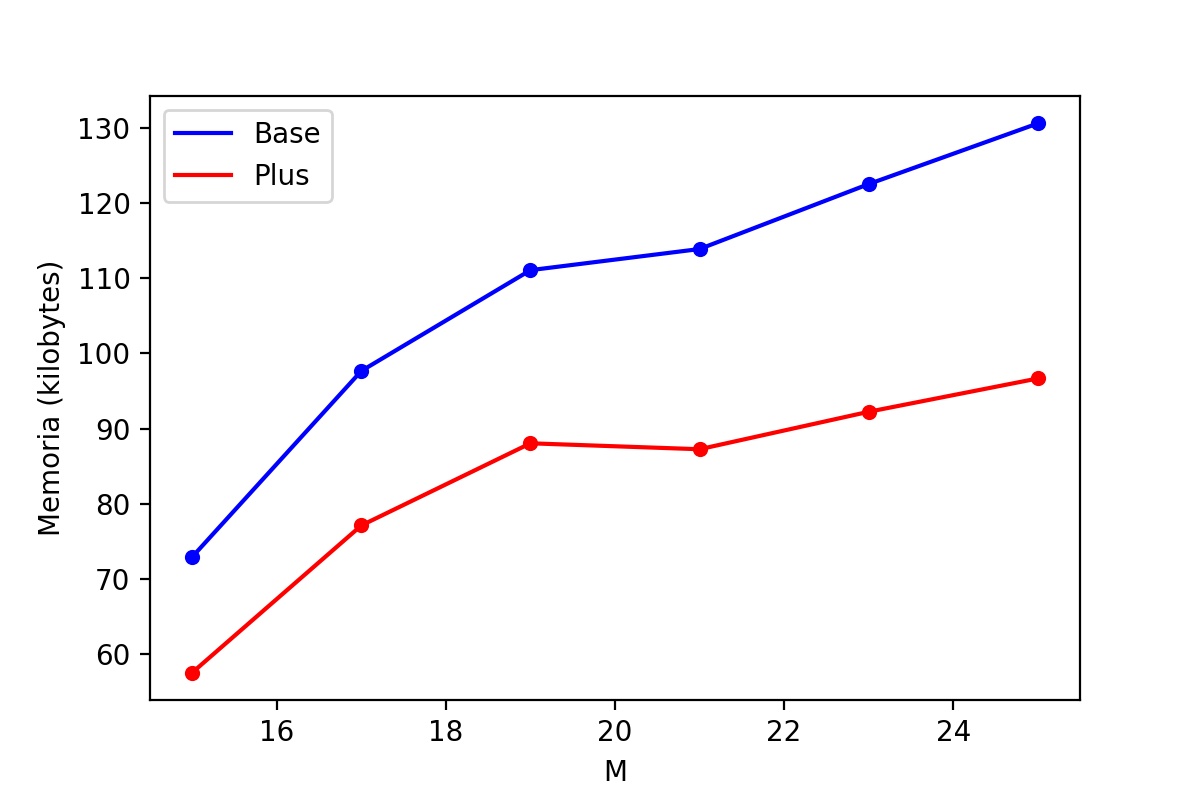
\includegraphics[width=0.8\linewidth]{figures/random/r_m_mem.png}
\caption{Occupazione spaziale dell'algoritmo al variare delle colonne di A}
\label{row:mem:r}
\end{figure}